\documentclass[12pt]{article}
\usepackage[margin=2.5cm]{geometry}
\usepackage{enumerate}
\usepackage{amsfonts}
\usepackage{amsmath}
\usepackage{fancyhdr}
\usepackage{amsmath}
\usepackage{amssymb}
\usepackage{amsthm}
\usepackage{mdframed}
\usepackage{graphicx}
\usepackage{subcaption}
\usepackage{adjustbox}
\usepackage{listings}
\usepackage{xcolor}
\usepackage{courier}
\usepackage[utf]{kotex}
\usepackage{hyperref}
\usepackage{soul}

\definecolor{codegreen}{rgb}{0,0.6,0}
\definecolor{codegray}{rgb}{0.5,0.5,0.5}
\definecolor{codepurple}{rgb}{0.58,0,0.82}
\definecolor{backcolour}{rgb}{0.95,0.95,0.92}

\lstdefinestyle{mystyle}{
    backgroundcolor=\color{backcolour},
    commentstyle=\color{codegreen},
    keywordstyle=\color{magenta},
    numberstyle=\tiny\color{codegray},
    stringstyle=\color{codepurple},
    basicstyle=\ttfamily\footnotesize,
    breakatwhitespace=false,
    breaklines=true,
    captionpos=b,
    keepspaces=true,
    numbers=left,
    numbersep=5pt,
    showspaces=false,
    showstringspaces=false,
    showtabs=false,
    tabsize=1
}

\lstset{style=mystyle}

\pagestyle{fancy}
\renewcommand{\headrulewidth}{0.4pt}
\lhead{CSC 369}
\rhead{Midterm 3 Solution}

\begin{document}
\title{CSC 369 Midterm 3 Solution}

\bigskip

\begin{enumerate}[1.]
    \item

    \begin{enumerate}[a)]

        \item
        Yes, they are part of system call's Application Programming Interface,
        and they are the only way to interact between computer program and OS kernel.
        \bigskip

        \begin{mdframed}
        \underline{\textbf{Correct Solution}}

        \bigskip

        \color{red}A system call \underline{traps} into the kernel so that priviliged
        instruction can be run. A function call jumps into another instruction in user-mode\color{black}
        \end{mdframed}

        \bigskip

        \underline{\textbf{Notes}}

        \begin{itemize}
            \item \textbf{Function Call}

            \begin{itemize}
                \item jumps into another instruction in user mode
            \end{itemize}

            \item \textbf{System Calls}
            \begin{itemize}
                \item Is issued by a client
                \item \underline{traps} into the kernel so that priviliged instruction can be run
                \item Is the only entry points into the kernel system
                \item Provides services via API or Application Program Interface
                \item Has five different types of calls

                \begin{center}
                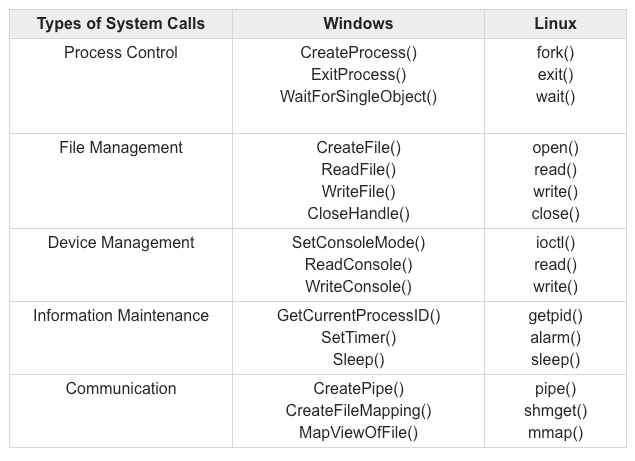
\includegraphics[width=0.8\linewidth]{../images/midterm_3_solution_1.png}
                \end{center}
            \end{itemize}

            \bigskip

            \underline{\textbf{Example}}

            \bigskip

            \texttt{open()}, \texttt{read()}, \texttt{write()}, \texttt{close()}, \texttt{mkdir()} are other examples of system calls
        \end{itemize}

        \bigskip

        \underline{\textbf{References}}

        \begin{enumerate}[1)]
            \item Tutorials Point, Types of System Calls, \href{https://www.tutorialspoint.com/different-types-of-system-calls}{link}
        \end{enumerate}

        \item

        It is user's responsibility to keep track of allocated blocks of heap memory,
        and memory leak occurs if user fails to deallocate allocated blocks of heap memory


        \bigskip

        \underline{\textbf{Notes}}

        \begin{itemize}
            \item \textbf{Memory API}

            \begin{itemize}
                \item Has two types of memory

                \begin{enumerate}[1.]
                    \item \textbf{Stack}

                    \begin{itemize}
                        \item Is also called \textbf{automatic memory}
                        \item Allocations and deallocations are managed by compiler
                        \item Deallocates memory by the end of function call
                    \end{itemize}

                    \item \textbf{Heap}

                    \begin{itemize}
                        \item Is long-lived
                        \item Allocation and deallocation are managed by user
                        \item Creates \textbf{memory leak} if memory not freed
                        \item \textbf{valgrind} is a useful heap memoery debugging tool \href{https://www.valgrind.org/docs/manual/quick-start.html}{link}
                    \end{itemize}
                \end{enumerate}

                \item \texttt{malloc()}
                \begin{itemize}
                    \item Is a C library call
                    \item \textbf{Syntax:} \texttt{void *malloc(size\_t size)}
                    \item Allocates a block of \texttt{size} bytes to \textbf{heap memory}
                    and if successful, returns a pointer to it
                    \item Returns \texttt{NULL} if memory allocation is unsuccessful
                \end{itemize}

                \bigskip

                \underline{\textbf{Example}}

                \bigskip

                \texttt{int *x = malloc(10 * sizeof(int));}

                \bigskip
                \item \texttt{free()}
                \begin{itemize}
                    \item Is a C library call
                    \item Frees heap memory that is no longer in use
                \end{itemize}

                \bigskip

                \underline{\textbf{Example}}

                \bigskip

                \texttt{int *x = malloc(10 * sizeof(int));}\\
                \texttt{...}\\
                \texttt{free(x);}

                \bigskip

                \item \texttt{brk(), sbrk(), mmap()}

                \begin{itemize}
                    \item Are system calls for memory management
                \end{itemize}

            \end{itemize}

            \item \textbf{Buffer overflow}
            \begin{itemize}
                \item is an error that occurs when not enough heap memory is allocated

                \bigskip

                \begin{center}
                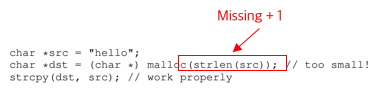
\includegraphics[width=0.8\linewidth]{../images/midterm_3_solution_2.png}
                \end{center}
            \end{itemize}
        \end{itemize}

        \item

        If the access by two threads are both about reading the stored value (as opposed to write),
        then concurrency error will not occur.

        \item

        Hand-over-hand locking is a fine-grained-locking, which allows more threads
        to be locked at once than single lock, and this means it will perform better
        than single lock when there is a lot of contention,

        \bigskip

        \underline{\textbf{Notes}}

        \begin{itemize}
            \item \textbf{Coarse-grained-locking}

            \begin{itemize}
                \item Is one big lock that is used any time any critical section is accessed
                \item Is easy to write
                \item Is easy to prove correctness
                \item No fault-tolerance but deadlock-free
                \item Perfoms poorly when contention (the need for performance due to load) is high
                \begin{itemize}
                    \item No concurrent access
                \end{itemize}

                \bigskip

                \underline{\textbf{Example}}

                \bigskip

                \begin{center}
                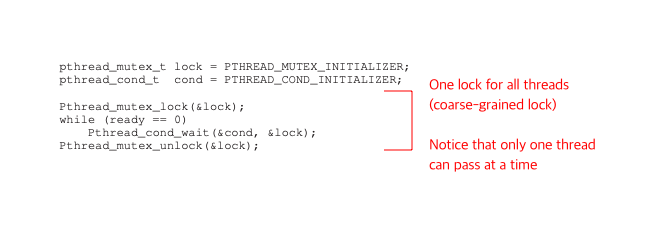
\includegraphics[width=\linewidth]{../images/midterm_3_solution_10.png}
                \end{center}
            \end{itemize}
            \item \textbf{Fine-grained-locking}

            \begin{itemize}
                \item Uses different locks to often protect different data and data strutures
                \item Allows more threads to be in locked code at once

                \bigskip

                \underline{\textbf{Example}}

                \bigskip

                \begin{center}
                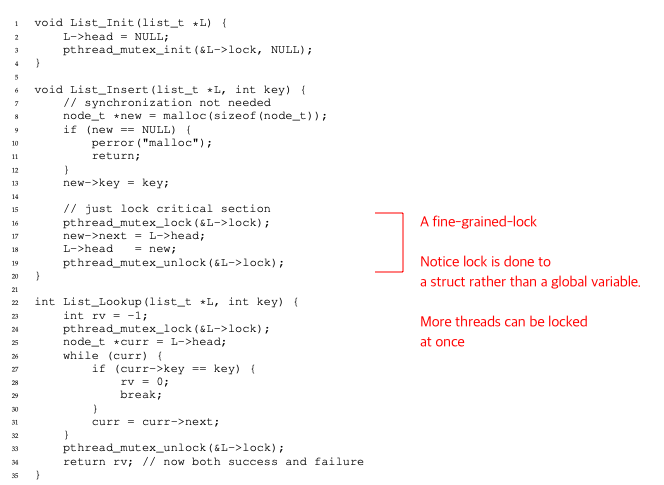
\includegraphics[width=\linewidth]{../images/midterm_3_solution_11.png}
                \end{center}

            \end{itemize}
            \item \textbf{Hand-over-hand locking}

            \begin{itemize}
                \item Idea: instead of having a single lock for the entire list, a lock per node
                of the list is added; when traversing the list, the list grabs the next node's lock,
                and releases the current node's lock
                \item Is a fine-grained-locking
                \item Holds at most 2 locks at a time

                \bigskip

                \underline{\textbf{Example}}

                \bigskip

                \begin{center}
                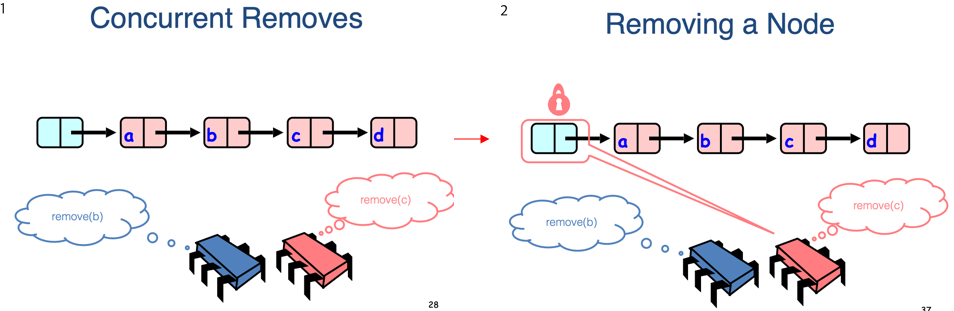
\includegraphics[width=\linewidth]{../images/midterm_3_solution_3.png}
                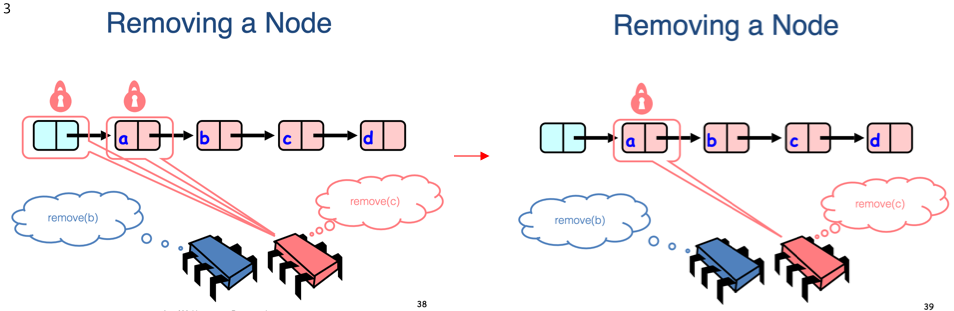
\includegraphics[width=\linewidth]{../images/midterm_3_solution_4.png}
                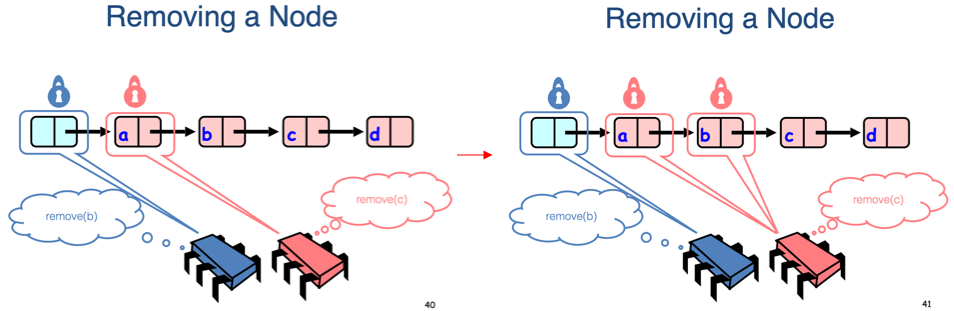
\includegraphics[width=\linewidth]{../images/midterm_3_solution_5.png}
                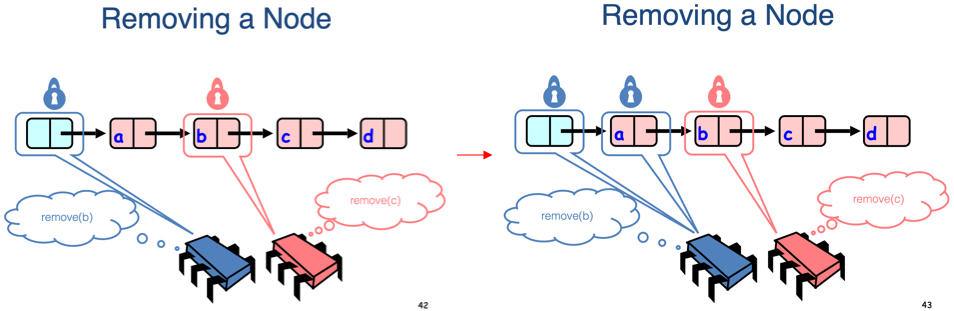
\includegraphics[width=\linewidth]{../images/midterm_3_solution_6.png}
                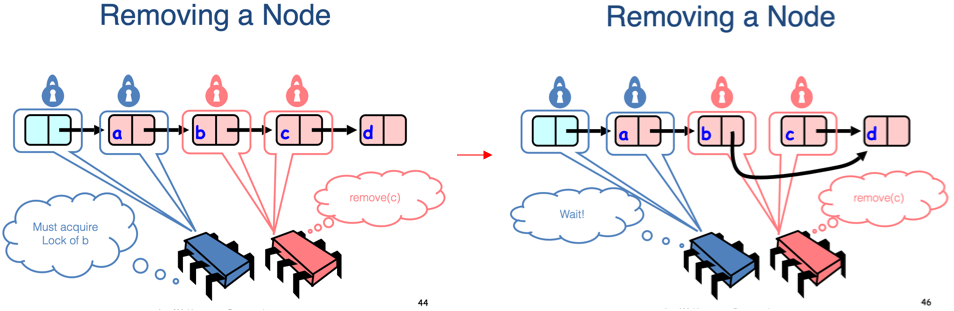
\includegraphics[width=\linewidth]{../images/midterm_3_solution_7.png}
                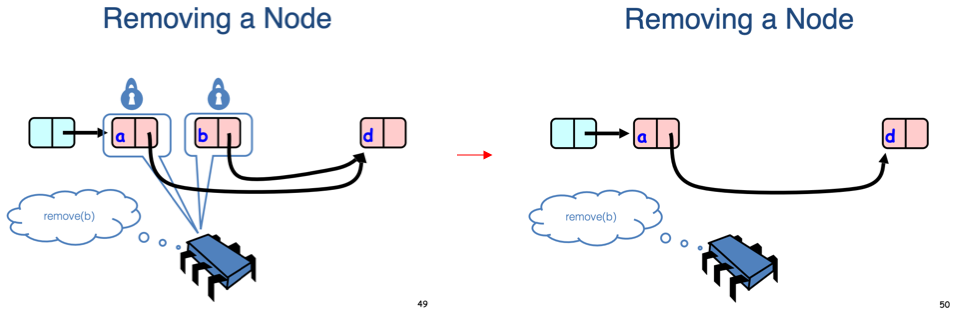
\includegraphics[width=\linewidth]{../images/midterm_3_solution_8.png}
                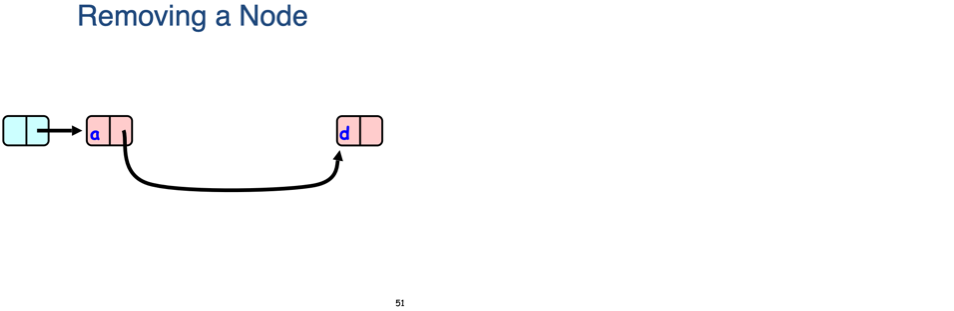
\includegraphics[width=\linewidth]{../images/midterm_3_solution_9.png}
                \end{center}

            \end{itemize}
        \end{itemize}

        \bigskip

        \underline{\textbf{References}}

        \begin{enumerate}[1)]
            \item Techion, Linked Lists: The Role of Locking, \href{http://www.cs.technion.ac.il/~erez/courses/seminar/talks/05.pdf}{link}
        \end{enumerate}

        \item

        \bigskip

        Interactive systems emphasizes quick response time, and for non-preemtive
        scheduling algorithms, the shorter tasks must wait for a process to finish,
        which means poor response time.

        \bigskip

        \underline{\textbf{Notes}}

        \begin{itemize}
            \item \textbf{Preemtive Scheduling Algorihtm}

            \begin{itemize}
                \item Are designed so that different processes can be executed in the
                middle of any current process execution.
                \item Today, all of the modern scheduling algorithms are \textbf{preemptive}

                \bigskip

                \underline{\textbf{Example}}

                \bigskip

                Shortest-Time-To-Completion (STCF) Scheduler

                \bigskip
            \end{itemize}
            \item \textbf{Non-preemtive Scheduling Algorithm}

            \begin{itemize}
                \item Are designed so that once a process enters the running state,
                it cannot be preempted (forestalled) until it completes its allotted time

                \bigskip

                \underline{\textbf{Example}}

                \bigskip

                Shortest Job First (SJF) scheduler
            \end{itemize}
        \end{itemize}

        \item

        Round Robin uses time slice on each process such that it returns
        quicker response time than Shortest Time to Completion First scheduling algorithm

        \item

        Trap instruction is a non-previleged operation performed in user mode that
        raises system's previlege level to kernel mode.

        \bigskip

        \underline{\textbf{Notes}}

        \begin{itemize}
            \item \textbf{Trap}
            \begin{itemize}
                \item Is an exception in a user process $^{[1]}$
                \item Is an interrupt caused by an exceptional condition (breakpoint, division by zero, invalid memory access) $^{[2]}$
                \item Usually results in kernel mode by invoking \textbf{trap instruction}$^{[2]}$
            \end{itemize}

            \item \textbf{Trap Instruction}

            \begin{itemize}
                \item when \textbf{Trap} or \textbf{System call} is invoked, \textbf{Trap instruction}
                simultaneously jumps into the kernel and raise the previlege
                level to kernel mode
            \end{itemize}
        \end{itemize}

    \end{enumerate}





\end{enumerate}

\end{document}